\section{Heurs}

\begin{center}
    \includegraphics{heur1}
\end{center}

\textbf{Formelle:} Il est vingt heures dix.

\begin{center}
\includegraphics{heur2}
\end{center}

\textbf{Formelle:} Il est midi cinquante-neuf.

\textbf{Informelle:} Il est treze heurs moins un.

\begin{center}
    \includegraphics{heur3}
\end{center}

\textbf{Formelle:} Il est quatre heures quarante-cinq.

\textbf{Informelle:} Il est cinq heures moins quinze.

\begin{center}
    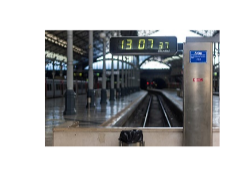
\includegraphics{heur4}
\end{center}

\textbf{Formelle:} Il est treze heures sept.

\begin{center}
    \includegraphics{heur5}
\end{center}

\textbf{Formelle:} Il est minuit. / Il est vingt-quatre heurs.

\begin{center}
    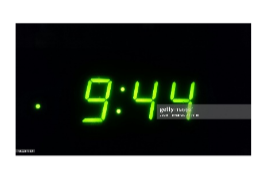
\includegraphics{heur6}
\end{center}

\textbf{Formelle:} Il est neuf heurs quarante-quatre.

\textbf{Informelle:} Il est dix heurs moins seize.

\begin{center}
    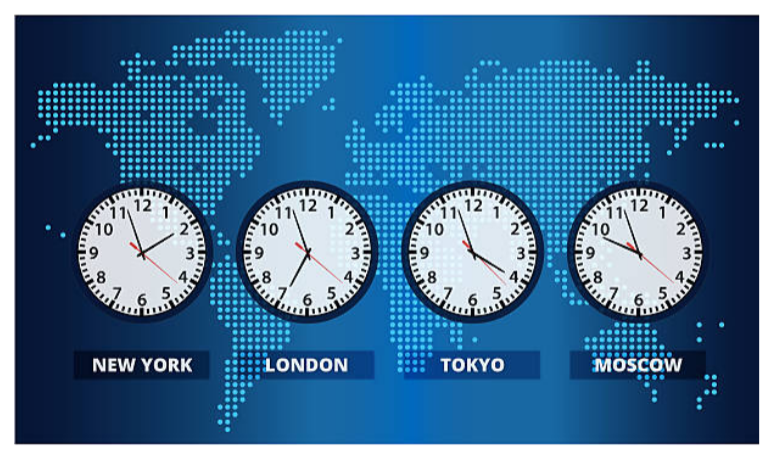
\includegraphics[scale=0.4]{heur7}
\end{center}

\textbf{Formelle:} 

\textbf{Informelle:}

\begin{center}
    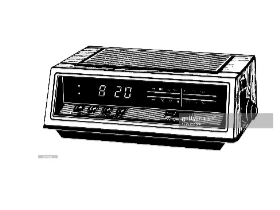
\includegraphics{heur8}
\end{center}

\textbf{Formelle:} Il est huit heurs vingt.

\begin{center}
    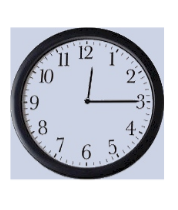
\includegraphics{heur9}
\end{center}

\textbf{Formelle:} Il est midi quinze. / Il est douze heurs quinze. 

\begin{center}
    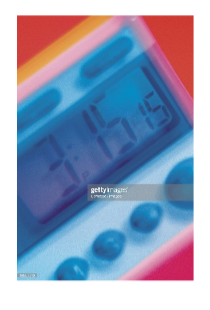
\includegraphics{heur10}
\end{center}

\textbf{Formelle:} Il est trois heurs quinze.